\begin{frame}
  \begin{tikzpicture}
    \begin{axis}[ xbar=0pt, /pgf/bar shift=0pt, legend style={ legend columns=4,
        at={(xticklabel cs:0.5)}, anchor=north, draw=none }, ytick={0,...,15},
      ytick style={draw=none},% <- added
      axis y line*=none, axis x line*=bottom, tick label
      style={font=\footnotesize}, legend style={font=\footnotesize}, label
      style={font=\footnotesize}, xtick style={draw=none},% <- added
      xtick={0,1,...,12}, width=.9\textwidth, bar width=3mm, y dir = reverse,
      xmin=0, xmax=13, area legend,
      y=5mm, enlarge y limits={abs=0.625},
      style={text=black}, every axis plot/.append style={fill},
      nodes near coords, nodes near coords,
      yticklabels={%
        {\topicref{Grenseverdier}},
        {\topicref{Gradient}},
        {\topicref{Epsilon-delta}},
        {\topicref{Kjerneregelen}},
        {\topicref{Taylor-approksimasjon}},
        {\topicref{Tangenter}},
        {\topicref{Kritiske-punkter}},
        {\topicref{Optimering}},
        {\topicref{Linjeintegral}},
        {\topicref{Konservative-vektorfelt}},
        {\topicref{Dobbelintegraler}},
        {\topicref{Integrasjonsrekkefolge}},
        {\topicref{Trippelintegral}},
        {\topicref{Greens-teorem}},
        {\topicref{Divergensteoremet}},
        {\topicref{Stokes-teorem}}}]
      \addplot[fill=gray] coordinates {(8,0)};
      \addplot[fill=gray] coordinates {(4,1)};
      \addplot[fill=gray] coordinates {(1,2)};
      \addplot[fill=gray] coordinates {(7,3)};
      \addplot[fill=gray] coordinates {(1,4)};
      \addplot[fill=gray] coordinates {(7,5)};
      \addplot[fill=gray] coordinates {(11,6)};
      \addplot[fill=gray] coordinates {(4,7)};
      \addplot[fill=gray] coordinates {(3,8)};
      \addplot[fill=gray] coordinates {(8,9)};
      \addplot[fill=gray] coordinates {(7,10)};
      \addplot[fill=gray] coordinates {(3,11)};
      \addplot[fill=gray] coordinates {(4,12)};
      \addplot[fill=gray] coordinates {(4,13)};
      \addplot[fill=gray] coordinates {(8,14)};
      \addplot[fill=dgreen] coordinates {(6,15)};
    \end{axis}
  \end{tikzpicture}
\end{frame}

\begin{frame}
  \subsection{Stokes-teorem}\label{subsec:Stokes-teorem}
  \frametitle{Stokes-teorem}
  \centerline{%
    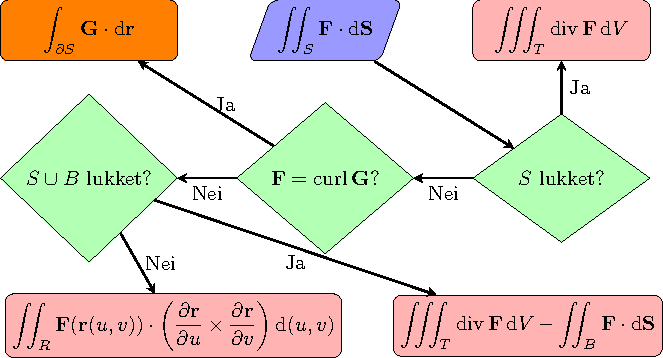
\includegraphics{../img/flytskjema-overflateintegral-2}
  }

\end{frame}
\begin{frame}
\begin{theorem}[Stokes' teorem]
  La $S$ være en orienterbar glatt overflate som er begrenset av en enkel,
  lukket stykkevis-glatt randkurve $C$ med positiv orientasjon. Dersom $\F$ er
  et vektorfelt med kontinuerlige partiellderiverte på $S$ så er
  \begin{equation*}
    \iint_S \curl \F \cdot \dSS = \int_C \F \cdot \dr.
  \end{equation*}
\end{theorem}
\centerline{
  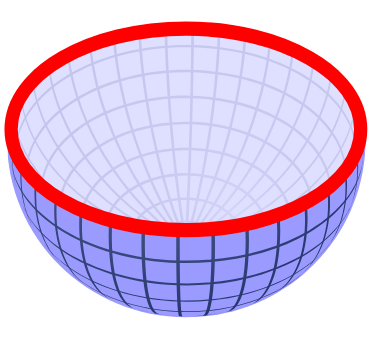
\includegraphics[scale=0.5]{../img/stokes-surface.png}
}
\end{frame}

\begin{frame}
  \begin{oppgave}{K2012, Oppgave 6c}
    Legemet $T$ er avgrenset av paraboloiden $z = 4x^2 +4y^2$ og planet $z = 4$.
    La $S$ være den delen av overflaten til $T$ som ligger på paraboloiden $z =
    4x^2 + 4y^2$ , og la $\vek{n}$ være enhetsnormalen til $S$ som peker ut av
    legemet $T$ . Vektorfeltet $F$ er
$
  \F(x, y, z) = \frac{yz}{8\pi}\I - \frac{x}{2\pi} \J + \frac{z}{4}\K
$. Regn ut
\begin{equation*}
  \iint_S \curl \F \cdot \vek{n} \dS.
\end{equation*}
\end{oppgave}
\end{frame}
\begin{frame}
\centerline{%
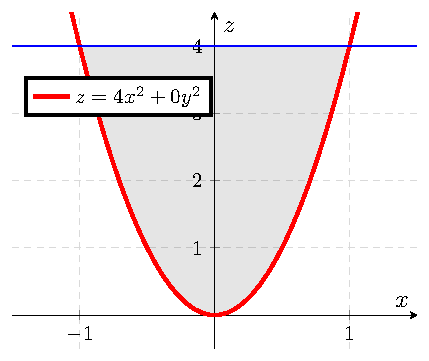
\includegraphics[width=0.4\textwidth]{../img/stokes-xz}%
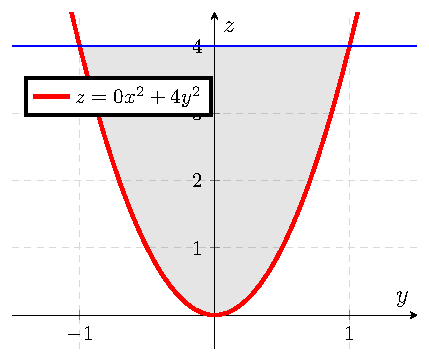
\includegraphics[width=0.4\textwidth]{../img/stokes-yz}}
\centerline{%
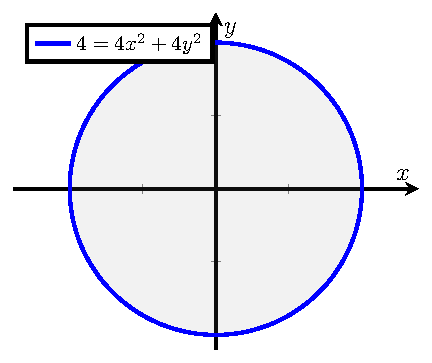
\includegraphics[width=0.4\textwidth]{../img/stokes-xy}%
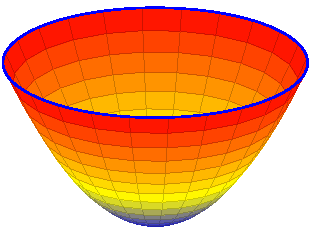
\includegraphics[width=0.4\textwidth]{../img/stokes-3d}}
\end{frame}

\begin{frame}
  \begin{oppgave}{K2012, Oppgave 6c}
    Legemet $T$ er avgrenset av paraboloiden $z = 4x^2 +4y^2$ og planet $z = 4$.
    La $S$ være den delen av overflaten til $T$ som ligger på paraboloiden $z =
    4x^2 + 4y^2$ , og la $\vek{n}$ være enhetsnormalen til $S$ som peker ut av
    legemet $T$ . Vektorfeltet $F$ er
$
  \F(x, y, z) = \frac{yz}{8\pi}\I - \frac{x}{2\pi} \J + \frac{z}{4}\K
$. Regn ut
\begin{equation*}
  \iint_S \curl \F \cdot \vek{n} \dS.
\end{equation*}
\end{oppgave}

\only<1->{
Flatene $z = 4x^2 + 4z^2$ og $z = 4$ skjærer hverandre i sirkelen $x^2 + y^2 =
1$, $z = 4$. }\only<2->{Randen til legemet $T$ er altså sirkelen med radius $r =
1$ og $z = 4$, som vi kaller $C$. Vi ønsker å beregne fluxen ut av det
\textcolor{red}{røde} området fra forrige side. Normalvektoren peker ut av
legemet, altså
\emph{nedover} og vi må parametrisere randen $C$ \emph{med}-klokken og ikke mot
som vanlig.
\begin{equation*}
  \rr(\theta) = (\sin \theta) \I + (\cos \theta) \J + 4 \K
\end{equation*}}
\only<7>{
\vspace{-0.5cm}
  \begin{equation*}
  \iint_S \curl \F \cdot \vek{n} \dS =
  \int_C \F \cdot \dr= 1
\end{equation*}}
\visible<3-6>{
  \vspace{-0.5cm}
\begin{equation*}
  \int_C \F \cdot \dr
  \only<3>{= \int_0^{2\pi} (\frac{4(\cos t)}{8\pi}, -\frac{\sin t}{2\pi}, 1)(\cos t, -\sin t, 0) \dt}
  \only<4->{= \frac{1}{2\pi}\int_0^{2\pi} (\cos t)^2 + (\sin t)^2 \dt}
  \visible<5->{= \frac{1}{2\pi}\int_0^{2\pi} 1 \dt}
  \visible<6>{= 1}
\end{equation*}}

\end{frame}

%%% Local Variables:
%%% mode: latex
%%% TeX-master: "main"
%%% End:
